\section{\textit{Web Services} em Ambientes de TV Digital Interativa}

Como visto no Capítulo \ref{cap:ws}, a tecnologia de \textit{Web Services} permite a integração entre sistemas heterogêneos, de uma forma simples e padronizada, utilizando protocolos e padrões já estabelecidos na Web. Com a TV Digital Interativa (TVDI) não é diferente, o uso dos \textit{Web Services} traz muitas facilidades e benefícios. Pelo fato de aplicações de TV Digital (TVD) serem principalmente implementadas em um modelo \textit{desktop}, e pela baixa capacidade de recursos dos receptor de TVD, os \textit{Set-top boxes}, a construção de aplicações distribuídas com uso de \textit{Web Services} libera o receptor de realizar processamentos pesados, que podem ser delegados a um WS. Desta forma, o uso dos WSs permite ainda, que as aplicações de TVD que fazem uso desta tecnologia, tenham um tamanho reduzido, devido às regras de negócio serem implementadas no WS, necessitando de menos largura e banda para transmitir as mesmas, e menor espaço em memória para armazená-las.

Tendo em vista os benefícios dos WSs para aplicações de TV Digital, algumas propostas surgem para provimento e descoberta de serviços em tal ambiente, como apresentado nas seções seguintes.

\subsection{Provendo WSs em Ambientes de TVD Móvel \cite{vilas2007providing}} %Providing WSs over DVB-H Mobile Virtual Web Services

Com o crescimento do acesso à Internet a partir de dispositivos móveis, tendência mundial também observada no Brasil 
\cite{banda-larga-movel-olhar-digital}, é cada vez mais comum o acesso a serviços a partir de tais dispositivos. No entanto, devido à reduzida capacidade da maioria destes dispositivos, as aplicações móveis acessadas a partir deles, devem ser tão simples quanto possível. Desta forma, o trabalho em \cite{vilas2007providing} apresenta um \textit{framework} para reduzir a complexidade de tais aplicações, criando \textit{Web Services} Virtuais. Estes são grupos de um ou mais serviços, permitindo que o dispositivo móvel possa utilizá-los, com transparência de localização dos serviços, além de permitir balanceamento de carga e resiliência.

Outro objetivo do trabalho apresentado em \cite{vilas2007providing}, é permitir a desvinculação das aplicações móveis de um provedor de serviços específico. Como, convencionalmente, aplicações clientes são atreladas a um determinado provedor, a complexidade de troca de provedor em tempo de execução pode ser excessiva para um dispositivo móvel. Além do mais, em dispositivos móveis, normalmente a troca do provedor de serviços requer a troca e reconfiguração da aplicação cliente, o que pode ser incômodo para o usuário.

Com isto, em \cite{vilas2007providing} é apresentada a proposta de \textit{Virtual Web Services} (VWSs)\nomenclature{VWS}{\textit{Virtual Web Service}}. Um VWS é um \textit{Web Service} padrão, que agrupa um ou mais serviços, criando uma camada de abstração entre os clientes móveis e os provedores de serviços, escondendo dos clientes a complexidade, disponibilidade e localização dos serviços. A Figura \ref{fig:virtual-ws} apresenta um cenário de uso de VWS.

\begin{center}
	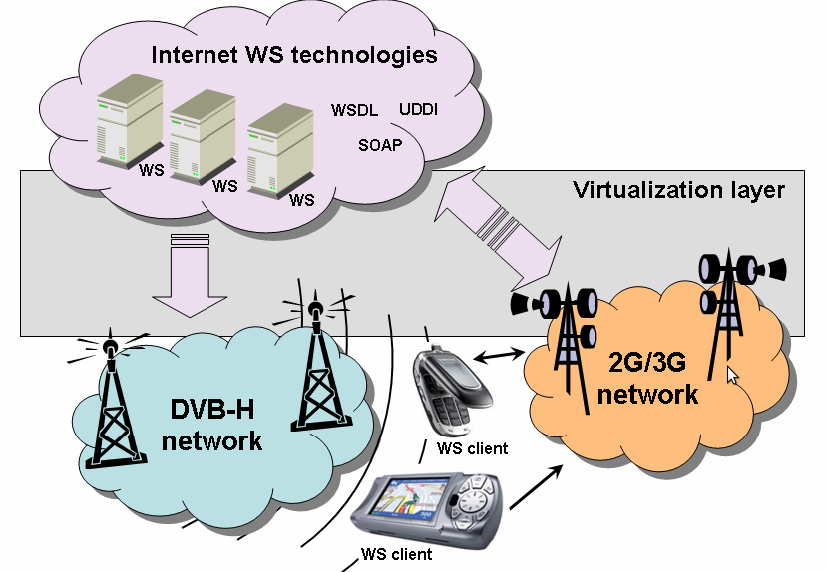
\includegraphics[width=0.8\textwidth]{images/virtual-ws-scenario.png}
	\captionof{figure}{Cenário de uso de um \textit{Virtual Web Service} \cite{vilas2007providing}}
	\label{fig:virtual-ws}
\end{center}

Diferentes provedores que fornecem um mesmo serviço, apesar de todos usarem XML para representar os dados trocados, podem receber diferentes tipos de parâmetros e devolver respostas em diferentes formatos. Em \cite{vilas2007providing} é apresentado um exemplo de serviço para obtenção das condições do tráfego em determinado local. Assim, um serviço pode fornecer as condições de fluxo do trânsito numa escola de 1 a 5, outro pode fornecer valores textuais como "Devagar", "Congestionado" e "Fluxo Livre". Desta forma, com o uso de VWS, as aplicações clientes não precisam se preocupar com estes detalhes de implementação de cada serviço. O VWS cria uma interface única para acesso aos diferentes serviços de informações de trânsito, sendo ele mesmo um \textit{Web Service} no padrão SOAP, que possui uma interface descrita por meio de um WSDL padrão.

Um VWS permite ainda a seleção de serviços baseada em fatores de QoS, permitindo ainda, a implementação de mecanismos de \textit{cache}. Tal mecanismo permite que resultados de invocações a um serviço sejam armazenadas no servidor do VWS, para que invocações futuras, usando os mesmos parâmetros de entrada, recebam o resultado já processado e armazenado previamente, podendo reduzindo o tempo de resposta das requisições em \textit{cache}.

\subsubsection{Conclusões}

A solução apresentada em \cite{vilas2007providing} é bastante relevante, por agrupar serviços similares, disponibilizados por diferentes provedores, em uma camada de abstração denominada \textit{Virtual Web Service}. Esta camada permite a seleção de serviços baseada em fatores de QoS, além de prover transparência de localização e resiliência. Outro ponto forte é o uso dos protocolos padrões de \textit{Web Services}, como HTTP, WSDL e SOAP. Desta forma, para as aplicações clientes, não há diferença entre um \textit{Virtual Web Service} e um \textit{Web Service} convencional.
